This section focuses on derivation of Bayesian inference algorithms for a variety of graphical models. The purpose of this section to practice derivation and implementation of Bayesian inference algorithms focusing on Markov-Chain Monte-Carlo (MCMC) sampling techniques from high dimensional posterior distributions. 

%TODO: note on markov chain techniques (why markov dependency between samples at all)

\subsection{MLE / MAP}
\subsubsection{Naive Bayes}
Consider discrete-valued features $x \in \{1,...,K\}^{D}$ where $D$ is the number of features and $K$ is the number of distinct values they can take on. The Naive Bayes model assumes conditional independence of random variables $x$ given the class labels $y$, i.e.
\begin{equation}
    p(x|y=c, \theta) = \prod_{j=1}^{D} p(x_j|y=c, \theta_{jc})
\end{equation}
The class conditional density above can take several forms: (1) Gaussian $N(x_j|\mu_{jc}, \sigma_{jc}^{2})$, (2) Bernoulli $\mathrm{Ber}(x_j|\mu_jc)$, (3) Categorical $\mathrm{Cat}(x_j|\mu_{jc})$.\\

Let's assume that we have a Bernoulli class conditional density, which means that $x_{i,j} \sim \mathrm{Ber}(x_{i,j}|\theta_{jc})$ are binary indicators for presence ($x_{i,j} = 1$) of word $j$ in document $i$ or absence ($x_{i,j} = 0$) of the word, parameterized by $\theta_{jc}$. Note that in the context of Naive Bayes classification of text, a data point $x_i = \{x_{i,1},...,x_{i,j},...,x_{i,D}\}$ is a document with $j=\{1,...,D\}$ features (vocabulary words) and an associated document class label $y_i$.\\

We can write down the joint as follows:
\begin{equation}
    p(x_i, y_i|\theta) = p(y_i|\pi) \prod_{j=1}^{D}p(x_{ij}|y_i=c,\theta_{jc}) = \prod_{c=1}^{C}\pi_{c}^{1[y_i = c]} \prod_{j=1}^{D}\prod_{c=1}^{C}p(x_{ij}|y_i=c,\theta_{jc})^{1[y_i = c]}
\end{equation}
As a result, the log-likelihood for the entire corpus is:
\begin{eqnarray}
    \log p(D|\theta) &=& \log \prod_{i=1}^{n} p(x_i, y_i|\theta) = \sum_{i=1}^{n} \log p(x_i, y_i|\theta) \nonumber \\
&=& \sum_{i=1}^{N}\sum_{c=1}^{C}1[y_i = c]\log \pi_c + \sum_{i=1}^{n}\sum_{j=1}^{D}\sum_{c=1}^{C}1[y_i = c]\log p(x_{ij}|y_i = c, \theta_{jc}) \nonumber \\
&=& \sum_{c=1}^{C}N_c \log \pi_c + \sum_{j=1}^{D} \sum_{c=1}^{C}\sum_{i:y_i = c} \log \mathrm{Ber}(x_{ij}|\theta_{jc}) 
\end{eqnarray}

There is a problem if some of the words have zero counts. To solve this problem, we can introduce a prior on our latent variables that acts as $\alpha$-smoothing. For simplicity, we'll use a factored prior:
\begin{equation}
     p(\theta) = p(\pi)\prod_{j=1}^{D}\prod_{c=1}^{C}p(\theta_{jc}) = \mathrm{Dir}(\alpha_1,...,\alpha_C)\prod_{j=1}^{D}\prod_{c=1}^{C}\mathrm{Beta}(\beta_0, \beta_1)
\end{equation}
Combining the factored prior with the factored likelihood, we get:
\begin{eqnarray}
    p(\theta|D) &=& p(\pi|D)\prod_{j=1}^{D}\prod_{c=1}^{C}p(\theta_{jc}|D) \nonumber \\
    &=& \mathrm{Dir(\pi|N_1+\alpha_1,...,N_C+\alpha_C)}\prod_{j=1}^{D}\prod_{c=1}^{C}\mathrm{Beta}(\theta_{jc}|(N_c - N_{jc}) + \beta_0, N_{jc} + \beta_1)
\end{eqnarray}
We can use Calculus to find MAP estimates of model parameters. For $\pi$, we want to maximize the Lagrangian:
\begin{equation}
    l(\pi, \lambda) = \log \prod_{c=1}^{C}\pi_{c}^{\alpha_k + N_k - 1} + \lambda \big(1-\sum_c \pi_c \big) = \sum_{c=1}^{C}(\alpha_c + N_c - 1) \log \pi_c + \lambda \big(1-\sum_c \pi_c \big)
\end{equation}
Taking partial derivative with respect to $\pi_c$, we get:
\begin{equation}
   \frac{\partial l(\pi, \lambda)}{\partial \pi_c} = \frac{\alpha_c + N_c - 1}{\pi_c} - \lambda = 0 \implies \lambda \pi_c = \alpha_c + N_c - 1
\end{equation}
Using the sum to 1 constraint:
\begin{equation}
    \lambda \sum_{c=1}^{C} \pi_c = \sum_{c=1}^{C} \alpha_c + N_c - 1 \implies \lambda = \alpha_0 +N - C
\end{equation}
Therefore, the MAP estimate is:
\begin{equation}
    \pi_c = \frac{N_c + \alpha_c - 1}{N + \sum_c \alpha_c - C}
\end{equation}
We can use a similar argument to derive the MAP estimate of $\theta_{jc}$. Taking the log of the posterior and isolating the term of interest, we can find the mode of the Beta distribution using Calculus and as a result the MAP estiamte is:
\begin{equation}
\theta_{jc} = \frac{N_c - N_{jc} + \beta_0 - 1}{N_c - N_{jc} + \beta_0 + N_{jc} + \beta_1 - 2} = \frac{N_c - N_{jc} + \beta_0 - 1}{N_c +\beta_0 + \beta_1 - 2}
\end{equation}
Note, if we set $\beta_0 = \beta_1 = 1$, we get the MLE estimate and if we set $\beta_0 = \beta_1 = 2$, we get add 1 Laplacian smoothing.\\

Learning the model parameters is the first step. We would like to next use the learned parameters to make a prediction about the class label of a test document. Using Bayes rule, we have: 
\begin{equation}
    p(y=c|x, D) \propto p(y=c|D) \prod_{j=1}^{D}p(x_j|y=c, D) 
\end{equation}
Substituting the distributions and taking the log, we get:
\begin{equation}
    \log p(y=c|x, D) \propto \log \hat{\pi}_c + \sum_{j=1}^{D}\bigg(1[x_{ij} = 1]\log \hat{\theta}_{jc} + 1[x_{ij} = 0]\log(1-\hat{\theta}_{jc})\bigg)
\end{equation}
Thus, we can plug-in the MAP estimates $\hat{\pi}_c$ and $\hat{\theta_{jc}}$ in the expression above to compute the log probability of class label for a new document.

\subsection{Expectation Maximization (EM)}

The EM algorithm provides a way of computing ML/MAP estimates when we have unobserved latent variables and/or missing data. EM exploits the fact that if the data were fully observed, then the ML/MAP estimates would be easy to compute. In particular, EM is an iterative algorithm which alternates between inferring the missing values given the parameters (E step) and then optimizing the parameters given filled in data (M step).\\ 

In the EM algorithm, we define the complete data log-likelihood $l_c(\theta)$ where $x_i$ are the observed random variables and $z_i$ are unobserved. Since we don't know $z_i$ we can't compute $p(x_i, z_i|\theta)$ but we can compute an expectation of $l_c(\theta)$ wrt to parameters $\theta^{(k-1)}$ from the previous iteration.  
\begin{equation}
    l_c(\theta) = \sum_{i=1}^{N}\log p(x_i, z_i|\theta) 
\end{equation}
The goal of the E-step is to compute $Q(\theta, \theta^{(k-1)})$ on which the ML/MAP estimates depend. The goal of the M-step is to re-compute $\theta$ by finding the ML/MAP estimates:
\begin{eqnarray}
   \mathrm{E-step} &:& Q(\theta, \theta^{(k-1)}) =  E_{\theta^{(k-1)}}\big[l_c(\theta)|D, \theta^{(k-1)}\big] \\
   \mathrm{M-step} &:& \theta^{(k)} = \arg \max_{\theta}Q(\theta, \theta^{(k-1)}) + \log p(\theta)
\end{eqnarray}

\subsubsection{Gaussian Mixture Model (GMM)}

To derive the EM algorithm for GMM, we first need to compute the expected complete data log-likelihood:
\begin{eqnarray}
    Q(\theta, \theta^{(k-1)}) &=& E\bigg[\sum_i \log p(x_i, z_i|\theta) \bigg] \nonumber \\
    &=& \sum_i E\bigg[ \log \bigg[\prod_{k=1}^{K}(\pi_k p(x_i|\theta_k))^{1[z_i=k]}\bigg]\bigg] \\
    &=& \sum_i \sum_k E\big[1[z_i = k]\big] \log \big[\pi_k p(x_i|\theta_k) \big] \\
    &=& \sum_i \sum_k p(z_i = k|x_i,\theta^{(k-1)}) \log \big[\pi_k p(x_i|\theta_k) \big] \\
    &=& \sum_i \sum_k r_{ik} \log \pi_k + \sum_i \sum_k r_{ik} \log p(x_i|\theta_k)
\end{eqnarray}
where $r_{ik} = p(z_i = k | x_i, \theta^{(k-1)})$ is the soft assignment of point $x_i$ to cluster $k$.\\

\textbf{E-step}. Given $\theta^{(k-1)}$, we want to compute the soft assignments:
\begin{eqnarray}
    r_{ik} = p(z_i=k|x_i, \theta^{(k-1)}) = \frac{p(z_i=k,x_i|\theta^{(k-1)})}{\sum_{k=1}^{K}p(z_i=k,x_i|\theta^{(k-1)})} = \frac{p(x_i|z_i=k, \theta^{(k-1)})\pi_k}{\sum_{k=1}^{K}p(x_i|z_i=k, \theta^{(k-1)})\pi_k}
\end{eqnarray}
where $\pi_k = p(z_i = k)$ are the mixture proportions.\\

\textbf{M-step}. In the M step, we maximize $Q$ with respect to model parameters $\pi$ and $\theta_k$. First, let's find $\pi$ that maximizes the Lagrangian:
\begin{equation}
    \frac{\partial Q}{\partial \pi_k} = \frac{\partial}{\partial \pi_k} \bigg[\sum_i \sum_k r_{ik} \log \pi_k + \lambda(1 - \sum_k \pi_k)\bigg] = \sum_i r_{ik} \frac{1}{\pi_k} - \lambda = 0
\end{equation}
Substituting the above expression into the constraint, we get
\begin{equation}
    \sum_k \pi_k = 1 \implies  \sum_k \frac{1}{\lambda}\sum_i r_{ik} = 1 \implies \lambda = 
    \sum_i \sum_k r_{ik} = \sum_i 1 = N 
\end{equation}
Therefore, $\pi_k = \frac{1}{\lambda}\sum_i r_{ik} = \frac{1}{N}\sum_i r_{ik}$. To find the optimum parameters $\theta_k = \{\mu_k, \Sigma_k\}$, we want to optimize the terms of $Q$ that depend on $\theta_k$:
\begin{eqnarray}
    l(\mu_k,\Sigma_k) &=& \sum_i r_{ik} \log p(x_i|\theta_k) \nonumber \\
    &\propto& -\frac{1}{2} \sum_i r_{ik} \bigg[\log|\Sigma_k| + (x_i - \mu_k)^{T}\Sigma_{k}^{-1}(x_i - \mu_k) \bigg] 
\end{eqnarray}
To find the optimimum $\mu_k$, we differentiate the above expression. First, focusing on the second term inside the sum, we can make a substitution $y_i = x_i - \mu_k$: 
\begin{equation}
    \frac{\partial}{\partial \mu_k} (x_i - \mu_k)^{T}\Sigma_{k}^{-1}(x_i - \mu_k) = \frac{\partial}{\partial y_i} y_i^{T} \Sigma^{-1} y_i \frac{\partial y_i}{\partial \mu_k} = -1 \times (\Sigma^{-1} + \Sigma^{-T})y_i 
\end{equation}
Substituting the above expression, we get:
\begin{equation}
    \frac{\partial}{\partial \mu_k} l(\mu_k, \Sigma_k) \propto -\frac{1}{2}\sum_i r_{ik}\bigg[-2\Sigma^{-1}(x_i - \mu_k)\bigg] = \Sigma^{-1} \sum_i r_{ik} (x_i - \mu_k) = 0
\end{equation}
which implies that
\begin{equation}
    \sum_i r_{ik}(x_i - \mu_k) = 0 \implies \mu_k = \frac{\sum_i r_{ik} x_i}{\sum_i r_{ik}} 
\end{equation}
To compute optimum $\Sigma_k$, we can use the trace identity:
\begin{equation}
    x^{T}Ax = \mathrm{tr}(x^{T}Ax) = \mathrm{tr}(xx^{T}A) = \mathrm{tr}(Axx^{T})
\end{equation}
Using $\Lambda = \Sigma^{-1}$ notation, we have:
\begin{eqnarray}
    l(\Lambda) &\propto& -\frac{1}{2}\sum_i r_{ik} \log|\Lambda| - \frac{1}{2}\sum_i r_{ik} \mathrm{tr}\bigg[(x_i-\mu)(x_i-\mu)^{T}\Lambda\bigg] \nonumber \\ 
    &=& -\frac{1}{2}\sum_i r_{ik} \log|\Lambda| - \frac{1}{2}\mathrm{tr}(S_{\mu}\Lambda) 
\end{eqnarray}
Taking matrix derivative, we get:
\begin{eqnarray}
    \frac{\partial l(\Lambda)}{\partial \Lambda} &=& -\frac{1}{2}\sum_i r_{ik} \Lambda^{-T} - \frac{1}{2}S_{\mu}^{T} = 0 \nonumber \\
    \Lambda^{-1}\sum_i r_{ik} &=& S_{\mu}^{T} \implies \Sigma = \frac{S_{\mu}^{T}}{\sum_i r_{ik}} \nonumber \\
    \Sigma &=& \frac{\sum_i r_{ik} (x_i - \mu_k)(x_i - \mu_k)^{T}}{\sum_i r_{ik}} = \frac{\sum_i r_{ik}x_i x_{i}^{T}}{\sum_i r_{ik}} - \mu_k \mu_{k}^{T}
\end{eqnarray}
These equations make intuitive sense, the mean of cluster $k$ is a weighted by $r_{ik}$ average of all points assigned to cluster $k$, while the covariance is the weighted empirical scatter matrix. 

\subsubsection{Latent Dirichlet Allocation (LDA)}

The EM algorithm maximizes the log-likelihood of the observed data:
\begin{equation}
   \theta^{\ast} = \arg \max_{\theta} \sum_{i=1}^{n} \log p(x_i|\theta) = \arg \max_{\theta} \sum_{i=1}^{n} \log \big[\sum_z p(x_i,z_i|\theta) \big]
\end{equation}
where $p(x_i, z_i|\theta)$ is the joint distribution between the observed words $x_i$ and unobserved (latent) asssignments $z_i$ parameterized by $\theta$. In the case of LDA topic model, $\theta = \{\theta_d, \beta_{w|z}\}$ where $\theta_d \sim \mathrm{Dir}(\alpha)$ are document level topic proportions and $\beta_{w|z} \sim \mathrm{Dir}(\eta)$ are corpus level topics.\\

\textbf{E step}. Given $\theta^{(k)}$, we want to find soft counts $n(z)$ and $n(w,z)$. First, we compute the posterior over the topic assignments:
\begin{equation}
    p(z|w, \theta^{(k)}) = \frac{p(z,w|\theta^{(k)})}{\sum_z p(z,w|\theta^{(k)})} = \frac{\theta_{z|d}\beta_{w|z}}{\sum_z \theta_{z|d}\beta_{w|z}}
\end{equation}
Given the posterior $p(z|w,\theta^{(k)})$, we can compute the soft counts:
\begin{eqnarray}
    n(z)   &=& \sum_{i=1}^{n_d} p(z|w_i,\theta^{(k)}) \\
    n(w,z) &=& \sum_{d=1}^{D}\sum_{i=1}^{n_d} p(z|w_i,\theta^{(k)})\delta(w, w_i) 
\end{eqnarray}
where $\delta(w, w_i)$ is an indicator which is equal to $1$ when $w=w_i$ and $0$ otherwise.

\textbf{M step}. Given the soft counts $n(z)$ and $n(w,z)$, we want to update $\theta^{(k)}$:
\begin{eqnarray}
    \theta_{z|d}^{(k+1)} &=& \frac{n(z)}{n_d} \\
    \beta_{w|z}^{(k+1)} &=& \frac{n(w,z)}{\sum_{w \in V} n(w,z)}
\end{eqnarray}
where $n_d$ is the total number of words in document $d$ and $V$ is our vocabulary. Thus, we can initialize $\theta^{(0)}$ at random and iterate between the E-step and the M-step until convergence. The EM algorithm may require several restarts to avoid local optima. As a result of several iterations, the log-likelihood of observed words under the topic model will increase.    

%\subsubsection{Bayesian Linear Regression}
%TODO: see section 9.3.4 Bishop for warm start

\subsection{Gibbs Sampling}

%TODO: see David Mackay's book on general intro to different sampling techniques / insighful explanations / pseudo-code (e.g. HMC) etc.

\subsubsection{Latent Dirichlet Allocation}

The LDA graphical model associates each word $w_{i,d}$ with a topic label $z_{i,d} \in \{1,2,...,K\}$. Each document is associated with topic proportions $\theta_d$. The topics $\phi_k$ are shared across all documents. The hyper-parameters $\alpha$ and $\eta$ define our rior knowledge of topic proportions and topics, respectively. The full generative model can be summarized as follows:
\begin{eqnarray}
    \theta_d | \alpha &\sim& \mathrm{Dir}(\alpha)\\
    z_{i,d} | \theta_d &\sim& \mathrm{Cat}(\theta_d)\\
    \phi_k | \eta &\sim& \mathrm{Dir}(\eta)\\
    w_{i,d}|z_{i,d}=k,\phi &\sim& \mathrm{Cat}(\phi_k)
\end{eqnarray}

In order to derive Gibbs sampling updates, we focus on the joint distribution $p(w, z) = p(w|z)p(z)$ and we analytically integrate out $\theta$ and $\phi$ parameters. This is known as \textit{collapsed Gibbs sampling} and it tends to be more efficient because we are sampling in a lower dimensional space. The process of sampling $z$ and integrating out $\theta$ is known as \textit{Rao-Blackwellization} named after the following theorem:
\begin{theorem}
(Rao-Blackwell) Let $z$ and $\theta$ be dependent random variables and $f(z,\theta)$ be some scalar function, then:
\begin{equation}
    \mathrm{var}_{z,\theta}\big[f(z,\theta)\big] \geq \mathrm{var}_z \big[E_\theta [f(z,\theta) | z]\big]
\end{equation}
\end{theorem}
\textbf{Joint distribution $p(w,z)$.}\newline
We proceed with collapsed Gibbs sampling as follows:
\begin{eqnarray}
   p(w,z;\alpha,\eta) &=& p(w|z)p(z) = \int p(w,\phi|z)d\phi \times \int p(z,\theta)d\theta \nonumber \\ 
   &=& \int p(w|\phi,z)p(\phi)d\phi \times \int p(z|\theta)p(\theta)d\theta = I_1 \times I_2 
\end{eqnarray}
Let's compute $I_2$ first. We know that,
\begin{equation}
    p(\theta) = \prod_{d=1}^{D} p(\theta_d|\alpha) = \prod_{d=1}^{D} \mathrm{Dir}(\theta_d|\alpha) = \prod_{d=1}^{D}\frac{1}{Z(\alpha)}\prod_{k=1}^{K}\theta_{d,k}^{\alpha - 1},~~~\mathrm{where}~~~ Z(\alpha) = \frac{\prod \Gamma(\alpha_i)}{\Gamma(\sum \alpha_i)}
\end{equation}
where we assume that $\alpha_1 = \alpha_2 = \cdots = \alpha_k = \alpha$. Similarly, let's write out the distribution for $p(z|\theta)$:
\begin{eqnarray}
    p(z|\theta) &=& \prod_{d=1}^{D}\prod_{j=1}^{N_d}p(z_{d,j}|\theta_d) = \prod_{d=1}^{D}\prod_{j=1}^{N_d}\mathrm{Cat}(\theta_d) = \prod_{d=1}^{D}\prod_{j=1}^{N_d}\theta_{d,k}^{x_{k}^{j}} \nonumber \\ 
    &=& \prod_{d=1}^{D}\prod_{k=1}^{K}\theta_{d,k}^{\sum_{j=1}^{N_d}x_{k}^{j}} = \prod_{d=1}^{D}\prod_{k=1}^{K}\theta_{d,k}^{n_{d,k}} 
\end{eqnarray}
where $n_{d,k}$ is a count of words in document $d$ assigned to topic $k$, and $x_{k}^{j}$ is a one-hot encoded vector indicating the presence of topic $k$ assigned to word $j$. Combining the equations above, we get the following expression for $I_2$:
\begin{eqnarray}
p(z) &=& \int p(z|\theta) p(\theta) d\theta = \int \bigg[\prod_{d=1}^{D}\prod_{k=1}^{K}\theta_{d,k}^{n_{d,k}}\bigg] \bigg[\prod_{d=1}^{D}\frac{1}{Z(\alpha)}\prod_{k=1}^{K}\theta_{d,k}^{\alpha - 1}\bigg] d\theta \nonumber \\
&=& \frac{1}{Z(\alpha)}\prod_{d=1}^{D}\bigg[ \int \prod_{k=1}^{K}\theta_{d,k}^{\alpha + n_{d,k} - 1} d\theta_d \bigg] = \frac{1}{Z(\alpha)}\prod_{d=1}^{D}Z(\alpha + n_{d,k})
\end{eqnarray}
where we used the identity for the Dirichlet distribution:
\begin{equation}
    \int \prod_{i=1}^{k} x_{i}^{\alpha_i - 1} dx = Z(\alpha) = \frac{\prod_{i=1}^{n}\Gamma(\alpha_i)}{\Gamma(\sum_i \alpha_i)}
\end{equation}
Let's compute $I_1$ next.
\begin{equation}
    p(\phi) = \prod_{k=1}^{K}p(\phi_k|\eta) = \prod_{k=1}^{K}\mathrm{Dir}(\phi_k|\eta) = \prod_{k=1}^{K}\frac{1}{Z(\eta)}\prod_{v=1}^{V}\phi_{k,v}^{\eta - 1}, ~~~\mathrm{where}~~~Z(\eta) = \frac{\prod \Gamma(\eta_i)}{\Gamma(\sum \eta_i)}
\end{equation}
where we assume that $\eta_1 = \eta_2 = \cdots = \eta_v = \eta$. Similarly, let's write out the distribution for $p(w|\phi, z)$:
\begin{eqnarray}
    p(w|\phi, z) &=& \prod_{d=1}^{D}\prod_{j=1}^{Nd} \prod_{k=1}^{K}p(w_{d,j}|\phi_k) =  \prod_{d=1}^{D}\prod_{j=1}^{Nd} \prod_{k=1}^{K} \mathrm{Cat}(\phi_k) \nonumber \\
&=& \prod_{d=1}^{D}\prod_{j=1}^{Nd} \prod_{k=1}^{K} \prod_{v=1}^{V} \phi_{k,v}^{x_{v}^{d,j}} = \prod_{k=1}^{K} \prod_{v=1}^{V} \phi_{k,v}^{\sum_d \sum_j x_{v}^{d,j}} =  \prod_{k=1}^{K} \prod_{v=1}^{V} \phi_{k,v}^{n_{k,v}}
\end{eqnarray}
where $n_{k,v}$ is a count of the number of times word $v$ was assigned to topic $k$, and $x_{v}^{d,j}$ is a one-hot encoded vector indicating the presence of word $v$ in document $d$ at word location $j$. Combining the equations above, we get the following expression for $I_1$:
\begin{eqnarray}
    p(w|z) &=& \int p(w|\phi, z) p(\phi) d\phi = \int \bigg[\prod_{k=1}^{K} \prod_{v=1}^{V} \phi_{k,v}^{n_{k,v}}\bigg] \bigg[\prod_{k=1}^{K}\frac{1}{Z(\eta)}\prod_{v=1}^{V}\phi_{k,v}^{\eta - 1} \bigg] \nonumber \\
&=& \frac{1}{Z(\eta)}\prod_{k=1}^{K}\bigg[\int \prod_{v=1}^{V}\phi_{k,v}^{n_{k,v}+\eta - 1}\bigg] = \frac{1}{Z(\eta)}\prod_{k=1}^{K}Z(\eta + n_{k,v})
\end{eqnarray}
Finally, taking a product of $I_1$ and $I_2$, we can compute the joint distribution:
\begin{equation}
    p(w, z) = p(w|z)p(z) = \bigg[\frac{1}{Z(\eta)}\prod_{k=1}^{K}Z(\eta + n_{k,v})\bigg] \bigg[\frac{1}{Z(\alpha)}\prod_{d=1}^{D}Z(\alpha + n_{d,k})\bigg]
\end{equation}
\textbf{Posterior of $\theta$ and $\phi$.}\newline
We have integrated out $\theta$ and $\phi$ for collapsed Gibbs sampling, however, we still need to obtain the posterior distribution over these latent variables. In the derivation below, we condition on the assignments $z_{d,j}$ to compute the posterior distribution:
\begin{eqnarray}
    p(\theta_d|z_d) &\propto& p(z_d|\theta_d)p(\theta_d) = \prod_{j=1}^{N_d}p(z_{d,j}|\theta_d)\prod_{k=1}^{K}\theta_{d,k}^{\alpha - 1} = \prod_{k=1}^{K}\theta_{d,k}^{n_{d,k}}\prod_{k=1}^{K}\theta_{d,k}^{\alpha - 1} \nonumber \\
    &=& \prod_{k=1}^{K}\theta_{d,k}^{n_{d,k}+\alpha - 1} \sim \mathrm{Dir}(\alpha + n_{d,k})
\end{eqnarray}
Similarly, $\phi_{k,v} \sim \mathrm{Dir}(\eta + n_{k,v})$.\\\\
\textbf{Collapsed Gibbs updates.}\newline
We need to compute the full conditional distribution $p(z_i|z_{-i}, w)$. We can proceed as follows:
\begin{eqnarray}
    p(z_i=k|z_{-i}, w) &=& \frac{p(z_i, z_{-i}, w)}{p(z_{-i}, w)} = \frac{p(w|z)p(z)}{p(z_{-i}, w_{-i}, w_i)} = \frac{p(w|z)p(z)}{p(w_{-i}|z_{-i},w_i)p(z_{-i})p(w_i)} \nonumber \\
    &\propto& \frac{p(w|z)p(z)}{p(w_{-i}|z_{-i})p(z_{-i})} = \frac{\prod_{k=1}^{K}Z(\eta + n_{k,v})}{\prod_{k=1}^{K}Z(\eta + n_{-k,v})} \times \frac{\prod_{d=1}^{D}Z(\alpha + n_{d,k})}{\prod_{d=1}^{D}Z(\alpha + n_{d,-k})}
\end{eqnarray}
For all docs other than $d=d^{\prime}$, the numerator and denominator of the second factor are exactly the same:
\begin{eqnarray}
     \frac{\prod_{d=1}^{D}Z(\alpha + n_{d,k})}{\prod_{d=1}^{D}Z(\alpha + n_{d,-k})} &=& \frac{Z(\alpha + n_{d^{\prime}, k})}{Z(\alpha + n_{d^{\prime}, -k})} = \frac{\prod_{k=1}^{K}\Gamma(\alpha + n_{d^{\prime}, k})}{\prod_{k=1}^{K}\Gamma(\alpha + n_{d^{\prime}, -k})} \times \frac{\Gamma(\sum_{k=1}^{K}\alpha + n_{d^{\prime},-k})}{\Gamma(\sum_{k=1}^{K}\alpha + n_{d^{\prime}, k})} \nonumber \\\ &=& \frac{\Gamma(\alpha + n_{d^{\prime}, -k^{\prime}} + 1)}{\Gamma(\alpha + n_{d^{\prime}, -k^{\prime}})} \times \frac{\Gamma(\sum_{k=1}^{K}\alpha + n_{d^{\prime},-k})}{\Gamma(\sum_{k=1}^{K}\alpha + n_{d^{\prime}, -k} + 1)} \nonumber \\
   &=& \frac{\alpha + n_{d^{\prime}, -k^{\prime}}}{\sum_{k=1}^{K}\alpha + n_{d^{\prime},-k}}
\end{eqnarray}
where we used the identity: $\Gamma(x+1) = x! = x(x-1)! = x\Gamma(x)$. Similarly, we can simplify the first factor to:
\begin{equation}
    \frac{\prod_{k=1}^{K}Z(\eta + n_{k,v})}{\prod_{k=1}^{K}Z(\eta + n_{-k,v})} = \frac{\eta + n_{-k^{\prime}, v^{\prime}}}{\sum_{v=1}^{V}\eta + n_{-k^{\prime}, v}}
\end{equation}
Putting the two factors together, our full conditional distribution is:
\begin{equation}
    p(z_i = k^{\prime}|z_{-i}, w) \propto \bigg[ \frac{\eta + n_{-k^{\prime},v^{\prime}}}{\sum_{v=1}^{V}\eta + n_{-k^{\prime}, v}} \bigg] \bigg[\frac{\alpha + n_{d^{\prime}, -k^{\prime}}}{\sum_{k=1}^{K}\alpha + n_{d^{\prime},-k}} \bigg]
\end{equation}
In the expression above, the first ratio is a probability of word $w_i$ (for which we are sampling the label $z_i$) under topic $k^{\prime}$ and the second ratio is the probability of topic $k^{\prime}$ in document $d^{\prime}$. 

\subsection{Metropolis-Hastings (MH) Sampling}
\subsubsection{Gaussian Mixture Model (GMM)}

\subsection{Slice sampling}
\subsection{HMC sampling}

%see Bishop for variational inference
\subsection{Annealed Importance Sampling}
Annealed Importance Sampling (AIS) is a method that combines independent importance sampling with Markov chain methods. It can be used to sample from multi-modal posterior distributions as well as to estimate ratios of normalizing constants (used in Bayesian model selection).

\subsubsection{AIS algorithm}

Consider a sequence of distributions $p_n(x), p_{n-1}(x),...,p_1(x), p_0(x)$, where $p_0(x)$ is our target distribution of interest (a posterior) and $p_n(x)$ is a starting distribution (a prior). Our goals is to draw samples from a multi-modal $p_0(x)$ by using a sequence of intermediate distributions $p_j(x)$:
\begin{equation}
    p_j(x) \propto p_0(x)^{\beta_j}p_n(x)^{1-\beta_j},~~~\mathrm{where}~~~ 0 = \beta_n < \beta_{n-1} < \cdots < \beta_{0} = 1
\end{equation}
We assume that we can draw samples from intermediate distributions $p_j(x)$ via a sequence of Markov chains $T_j(x, x^{\prime})$ that model a transition from state $x$ to $x^{\prime}$. $T_j(x, x^{\prime})$ can be any of the Markov chain methods that satisfy detailed balance, i.e. Gibbs, Slice or Metropolis-Hastings (MH) samplers. The AIS algorithm can be summarized as follows:

\begin{algorithm}
\caption{Annealed Importance Sampling (AIS) \cite{Neal1998}}
\label{alg:ais}
\begin{algorithmic}[1]
\STATE Define a target distribution $p_0(x)$, a prior $p_n(x)$, and an intermediate $p_j(x)$ 
\STATE Define a range of $\beta$ values: $0 = \beta_n < \beta_{n-1} < \cdots < \beta_{0} = 1$
\STATE Define the transitions $T_j(x,x^{\prime})$ 
\STATE \textbf{for} sample $s = 1$ to $S$ \textbf{do} 
\STATE ~~~ init $w = 0$
\STATE ~~~ sample $x_{prev} \sim p_n(x)$
\STATE ~~~ \textbf{for} $j=n-1$ to $1$:
\STATE ~~~ ~~~ $x_{new} \sim T_j(x_{prev}, \cdot)$ 
\STATE ~~~ ~~~ $x_{prev} = x_{new}$
\STATE ~~~ ~~~ $w = w + \log(p_{j-1}(x_{prev})) - \log(p_{j}(x_{prev}))$
\STATE ~~~ \textbf{end for}
\STATE ~~~ $\mathrm{samples}[s] = x_{prev}$
\STATE ~~~ $\mathrm{weights}[s] = \exp(w)$
\STATE \textbf{end for}
\STATE \textbf{return} samples, weights
\end{algorithmic}
\end{algorithm}
According to Algorithm \ref{alg:ais}, we obtain $1$ sample from the target $p_0(x)$ and the associated importance weight at the cost of $n$ samples from intermediate distributions $p_j(x)$. The algorithm is using an equation for computing the importance weights, let's derive it below.\\

AIS can be seen as importance sampling in an extended $z$-space $\{z_0,...,z_{n-1}\}$. We can represent the target distribution as follows:
\begin{equation}
    p(z) \propto f(z) = f_0(z_0)\tilde{T}_1(z_0, z_1)\tilde{T}_2(z_1, z_2)\times \cdots \times \tilde{T}_{n-1}(z_{n-2}, z_{n-1})
\end{equation}
where $\tilde{T}_{j}$ is the reversal of $T_j$. We assume the samples satisfy detailed balance:
\begin{eqnarray}
   p_j(z)\tilde{T}_{j}(z, z^{\prime}) &=& p_j(z^{\prime})T_{j}(z^{\prime}, z) \\
   \tilde{T}_{j}(z, z^{\prime}) &=& T_{j}(z^{\prime}, z)\frac{p_j(z^{\prime})}{p_{j}(z)} = T_{j}(z^{\prime}, z)\frac{f_j(z^{\prime})}{f_j(z)}
\end{eqnarray}
As a result, we can re-write the target distribution as follows:
\begin{equation}
   p(z) \propto f_0(z_0)\bigg[T_1(z_1, z_0)\frac{f_1(z_1)}{f_1(z_0)}\bigg]\bigg[T_2(z_2, z_1)\frac{f_2(z_2)}{f_2(z_1)}\bigg]\times ... \times \bigg[T_{n-1}(z_{n-1}, z_{n-2})\frac{f_{n-1}(z_{n-1})}{f_{n-1}(z_{n-2})}\bigg] 
\end{equation}
Similarly, the proposal distribution is given by:
\begin{equation}
    q(z) \propto g(z) = f_{n}(z_{n-1})T_{n-1}(z_{n-1}, z_{n-2})\times \cdots \times T_2(z_2, z_1)T_1(z_1, z_0)
\end{equation}
Thus, the importance weights are given by:
\begin{eqnarray}
    w &=& \frac{f(z_0,...,z_{n-1})}{g(z_0,...,z_{n-1})} \nonumber \\ 
      &=& \frac{f_0(z_0)\bigg[T_1(z_1, z_0)\frac{f_1(z_1)}{f_1(z_0)}\bigg]\bigg[T_2(z_2, z_1)\frac{f_2(z_2)}{f_2(z_1)}\bigg]\times \cdots \times \bigg[T_{n-1}(z_{n-1}, z_{n-2})\frac{f_{n-1}(z_{n-1})}{f_{n-1}(z_{n-2})}\bigg]}{T_1(z_1, z_0)T_2(z_2, z_1)\times \cdots \times T_{n-1}(z_{n-1}, z_{n-2})f_n(z_{n-1})} \nonumber \\
    &=& \frac{f_{n-1}(z_{n-1})}{f_n(z_{n-1})}\times \frac{f_{n-2}(z_{n-2})}{f_{n-1}(z_{n-2})}\times \cdots \times \frac{f_1(z_1)}{f_2(z_1)}\times \frac{f_0(z_0)}{f_1(z_0)}
\end{eqnarray}
We can see a telescoping product of ratios of distributions which is equal to standard importance sampling when $n=1$.\\ 

AIS can also be used to approximate the ratio of normalizing constants. Suppose, we are interested in computed an expected value of $f(x)$. We can proceed as follows:
\begin{eqnarray}
    E[f(x)] &=& \int f(x)p(x)dx = \int f(x)\frac{q(x)}{q(x)}p(x)dx = \frac{Z_q}{Z_p}\int f(x)\frac{\tilde{p}(x)}{\tilde{q}(x)}q(x)dx \nonumber \\
    &=& \frac{Z_q}{Z_p}\frac{1}{S}\sum_{s=1}^{S}\tilde{w}(s)f(s),~\mathrm{where}~s\sim q(x)~\mathrm{and}~\tilde{w}(s) = \frac{\tilde{p}(s)}{\tilde{q}(s)}
\end{eqnarray}
We can compute the ratio of normalizing constants as follows:
\begin{equation}
    \frac{Z_p}{Z_q} = \frac{1}{Z_q}\int \tilde{p}(x)dx = \frac{1}{Z_q}\int \frac{\tilde{p}(x)}{q(x)}q(x)dx = \int \frac{\tilde{p}(x)}{\tilde{q}(x)}q(x)dx = \frac{1}{S}\sum_{s=1}^{S}\tilde{w}(s)
\end{equation}
Combining the two expression above, we get:
\begin{equation}
    E[f] = \frac{Z_q}{Z_p}\frac{1}{S}\sum_{s=1}^{S}\tilde{w}(s)f(s) = \frac{\frac{1}{S}\sum_s \tilde{w}(s)f(s)}{\frac{1}{S}\sum_s \tilde{w}(s)} = \sum_{s=1}^{S}w(s)f(s)
\end{equation}

\subsubsection{AIS estimator}

This section studies the properties of AIS estimator and computes quantities relevant to characterizing the performance of AIS. The AIS estimator can be defined as follows:
\begin{equation}
    \hat{a} = E[a(x)] = \frac{\frac{1}{n}\sum_{i=1}^{n} \tilde{w}^{i}a(x_i)}{\frac{1}{n}\sum_{i=1}^{n}\tilde{w}^{i}} = \frac{1}{n}\sum_{i=1}^{n} w_{\ast}^{i}a(x_i),~~~\mathrm{where}~~~w_{\ast}^{i} = \tilde{w}^{i} / n^{-1}\sum_i \tilde{w}^{i}
\end{equation}
By the Weak Law of Large Numbers (WLLN), assuming independent samples $x_i$, we know that the average of iid samples converges in probability to the true mean:
\begin{equation}
   a = E[w_{\ast}(X_i)a(X_i)] \rightarrow b(\hat{a}) = E[\hat{a}] - a = 0
\end{equation}
where $X_i$ are assumed to be iid random variables distributed according to $q(x)$. As a result, AIS is in theory an unbiased estimator. However, due to samples from intermediate distributions being not always independent (due to correlations in Markov Chain using Metropolis-Hastings sampler), there can exist a bias associated with AIS estimates.\\

The variance of the AIS estimator is given by:
\begin{equation}
    \mathrm{VAR}(\hat{a}) = \frac{\sigma^2}{n} = \frac{1}{n}\frac{\sum_{i=1}^{n}\bigg(\tilde{w}^{i}(a(x_i) - \hat{a}) \bigg)^{2}}{\bigg(\sum_{i=1}^{n}\tilde{w}^{i}\bigg)^{2}}
\end{equation}
To check whether AIS estimate is consistent, we need to show that as we increase the number of samples $n$, the estimate $\hat{a}$ converges to the true value $a$ in probability:
\begin{equation}
    \lim_{n\rightarrow \infty} P(|\hat{a}_n - a| > \epsilon) = 0
\end{equation}
Using Chebyshev's inequality, we can bound the deviation from $a$ as follows:
\begin{equation}
    \lim_{n\rightarrow \infty} P(|\hat{a} - a| > \epsilon) \leq \frac{\mathrm{VAR}(\hat{a})}{\epsilon^2} = \frac{\sigma^2}{n \epsilon^2} = 0
\end{equation}
As a result, the AIS estimator is consistent, here we didn't need to use an assumption that samples are independent but we needed to assume that the variance of importance weights is finite. Thus, we expect the variance around the estimate to shrink as we add more samples. One factor that affects the variance of the estimator is the magnitude of importance weights. Since $w(x_i) = p(x_i)/q(x_i)$, the weights are small if $q(x_i)$ is similar to $p(x_i)$ and has heavy tails. This is the desired case that leads to a small variance in our estimate. 

We would like to have a way of telling when the importance weights are problematic, e.g. when only a couple of weights dominate the weighted sum. When samples are correlated the variance is $\sigma^2 / n_{eff}$, where $n_{eff}$ is the effective sample size. To compute an expression for effective sample size, we set the variance of weighted average equal to the variance of unweighted average:
\begin{equation}
    \mathrm{VAR}\bigg(\frac{1}{n}\sum_{i=1}^{n}a(x_i)\bigg) = \frac{\sigma^2}{n_{eff}} = \mathrm{VAR}\bigg(\frac{\frac{1}{n}\sum_{i=1}^{n}\tilde{w}^ia(x_i)}{\frac{1}{n}\sum_{i=1}^{n}\tilde{w}^{i}}\bigg)~~~\mathrm{where}~~~\mathrm{VAR}(a(x_i)) = \sigma^2
\end{equation}
Solving for $n_{eff}$, we get
\begin{equation}
    n_{eff} = \frac{(\sum_{i=1}^{n}w_i)^2}{\sum_{i=1}^{n}w_{i}^{2}} = \frac{n}{1 + \mathrm{VAR}(w_{\ast}^{i})} 
\end{equation}
We can use $n_{eff}$ is a kind of diagnostics for the importance sampler where the target number $n_{eff}$ depends on the application. We can also compute a confidence interval for our estimate. Given the variance expression above, an approximate 99\% confidence interval for $a$ is $\hat{a} \pm 2.58 \sigma_a / \sqrt{n}$.\\
%TODO: delta method + read more about IS / AIS estimator
%TODO: at some point want to get into NF!

\subsubsection{AIS experiments}

\textbf{Minimum Working Example}
%TODO describe experimental set-up + improvements (e.g. higher dimensional, multi-modal)
%TODO include ratio of normalizers estimation and MSE plot (see Qiang Liu's paper)
To test how well AIS can estimate the quantities of interest such as posterior mean and normalization constant, we design the following experiment. Let $p_n = N(0, 1)$ be the standard normal prior distribution and $p_0 \propto N(-5, 2)$ be the unnormalized posterior. We let $\beta$ linearly vary in the interval $[0, 1]$ divided into $100$ steps, i.e. we have $100$ intermediate distributions formed by taking a weighted geometric average between the prior and the posterior.

\begin{figure}[tbhp]
    \centering
    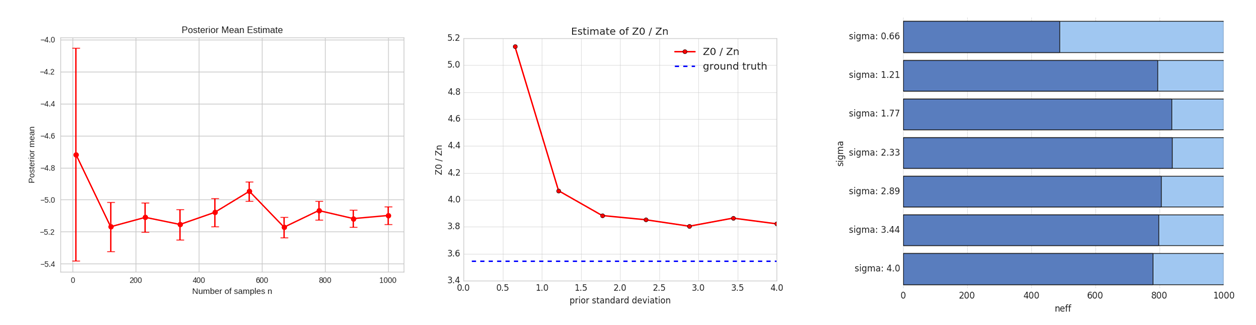
\includegraphics[width=\textwidth, trim={10 10 10 10}]{figures/ais_exp1.png}
    \caption{AIS posterior mean estimate (left). AIS normalizer estimate (middle). AIS effective sample size (right).}
    \label{fig:ais_exp1}
\end{figure}

We use $n=10$ step Metropolis-Hastings (MH) sampler to sample from intermediate distributions and compute importance weights as described in Algorithm \ref{alg:ais}. The experimental results are summarized in Figure \ref{fig:ais_exp1}. As expected, as the number of AIS samples increases the variance of our estimate drops. However, the AIS estimator is not completely unbiased as we can see from Figure \ref{fig:ais_exp1} (left) since the ground truth value is $-5$. Similarly, there's evidence of bias in the normalization constant estimate as can be seen in Figure \ref{fig:ais_exp1} (middle), since the ground truth value is equal to $Z_0/Z_n = \sqrt{4\pi} = 3.545$. This bias is most likely caused by the fact that samples are not completely independent (due to MH). We can also measure our sample efficiency by observing the number of effective samples Figure \ref{fig:ais_exp1} (right) as we vary the variance of our prior distribution. The solid bars indicate the effective number of samples out of a total of $1000$.  






